\section{Problem-Framing Scaffolds: Hot \& Cool Thinking \\in Creativity}
\label{sec:hats_exp}
Effective creative work requires both ``hot'' (exploratory) and ``cool'' (exploitative) thinking. Unfortunately, many people (especially novices) under-explore, jumping to the ``cool'' part too quickly, because they assume their current thinking ``has to be'' the path.  This paper presents empirical results of how metaphorical problem framing scaffolds can influence creative performance. The task used De Bono's ``Thinking Hats.'' In a between-subjects experiment comparing exploratory to exploitative problem frames, the exploratory problem frame led to more original designs and more diverse ideas during brainstorming. This work provides an empirical baseline of how -- even for short tasks -- assigning people responsibility for broad thinking leads to better creative work.

\subsection{Why are people so often averse to exploration?}
Problem-solving engages a cycle of ``hot'' (exploratory) and ``cool'' (exploitative) thinking, searching broadly before narrowing onto any single idea or solution \cite{kirkpatrick1983optimization,lucas2014children}(Figure \ref{fig:sim-ann}). People often \textit{satisfice}, stopping at the first solution they consider to be good enough \cite{simon1972theories}. Often, this is a savvy way to save time. However, the dark side of satisficing is when people underestimate the space of possibility, as often happens with complex creative problems, quickly settling on a path means forgoing (unconsidered) options that could be much better.  

\subsubsection{Strategies for Increasing Early Exploration Help to an Extent}

To encourage broader exploration early in problem-solving, brainstorming, process models like the Double Diamond, and design thinking approaches encourage wild ideas at the outset. Despite this explicit encouragement, people -- especially novices -- still under-explore. The tendency to cool too soon and fixate can be difficult to overcome. Iteration and examples alone do not necessarily mean greater divergence as people tend to explore within a narrow solution space \cite{Dow2009, jansson1991design, kulkarni2012early}. Without domain knowledge or strategies for exploration, people systematically underestimate how many better ideas are out there. 

% \begin{marginfigure}[5\baselineskip]
%   \begin{minipage}{\marginparwidth}
%     \vspace{-8cm}
%     \centering
%     \includegraphics[width=\marginparwidth]{images/green.png}
%      \includegraphics[width=\marginparwidth]{images/blue.png}
%     \caption{The green thinking hat represents exploration; the blue thinking hat represents exploitation.}

%     ~\label{fig:hats}
%   \end{minipage}
% \end{marginfigure}

\subsubsection{How Do We Overcome Satisficing?}
% \subsection{How Might We ``Set the Temperature'' of Creative Thought?}
We hypothesize that more explicitly attending to exploration and exploitation as phases may improve creativity. Approaches like brainstorming offer psychological safety and improve group's collective knowledge by ``encouraging wild ideas'' and ``deferring judgment.'' One potential advantage of design thinking and related methods is that seeing problems from a user's perspective and drawing inspiration from existing practices and challenges gives people a different vantage point from which to see ideas \cite{debono1985, Dow2009, teevan2017}. To \textit{harness} better ideas, one must first see them. Despite compelling advances from leading practitioners, the empirical basis for stretching people's horizons remains limited. 

This section explores the benefits of asking people to simply ``look further,'' and also provides a more cognitive account of process than is available in the practitioner literature. We present a between-subjects study comparing an explore problem-framing scaffold to an exploit problem-framing scaffold. We found that with an exploratory framing, people provide more original designs and show greater diversity of ideas during brainstorming. This section demonstrates how process scaffolds connect to design outcomes and can ``set the temperature'' in creative thinking. 

\subsection{Experiment 1: Can Problem-Framing Scaffolds Influence Creative Thought?}

\subsubsection{Method}
This between-subjects experiment establishes a baseline of whether it is possible to influence creative outcomes by scaffolding how to frame problems. We adapt our scaffolds from DeBono's \cite{debono1985} Thinking Hats. These ``hats'' provide a metaphor for particular roles and purviews. DeBono's Green Hat represents creativity and serves as our explore scaffold (Figure \ref{fig:hats}a); the Blue Hat represents action and goal-setting and serves as our exploit scaffold (Figure \ref{fig:hats}b). We hypothesized that the explore scaffold would lead to more original ideas and broader search during the brainstorming period while the exploit scaffold would lead to more practical, but less original ideas and narrower search during the brainstorming period.

\begin{figure}
\centering
  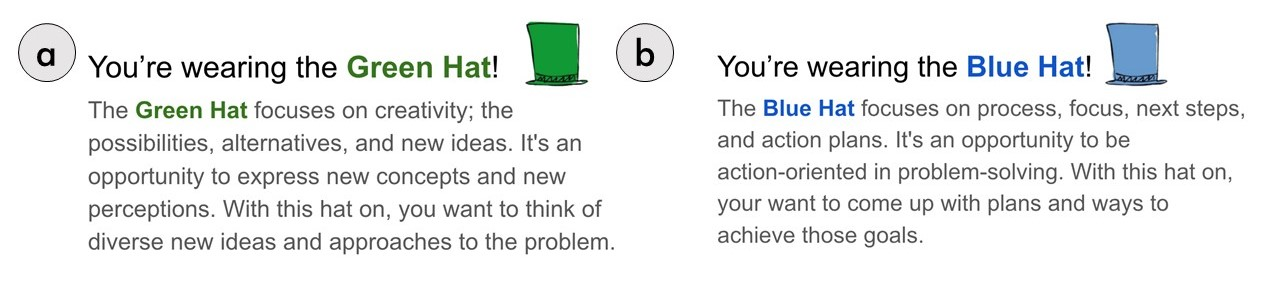
\includegraphics[width=\textwidth]{future/figures/thinking_hats.jpg}
  \caption{a) The green thinking hat represents exploration, and b) the blue thinking hat represents exploitation. Participants in Experiment 1 used these scaffolds during brainstorming.
}
  \label{fig:hats}
\end{figure}

34 participants (27 female) were recruited from the Psychology \& Cognitive Science subject pool (SONA) at a California research university. This task asked participants to redesign an aspect of the student eating experience to be better or more enjoyable. All participants received this scenario; half were randomly assigned to an \textit{Explore} frame, half to an \textit{Exploit} frame during the brainstorming period. The experiment gave five minutes for initial brainstorming and ten minutes to write a description of their preferred idea, why it is unique, and why it would improve the student eating experience. Lastly, a written survey asked participants questions about their experience with the Thinking Hat scaffolds.

\begin{figure}
\centering
  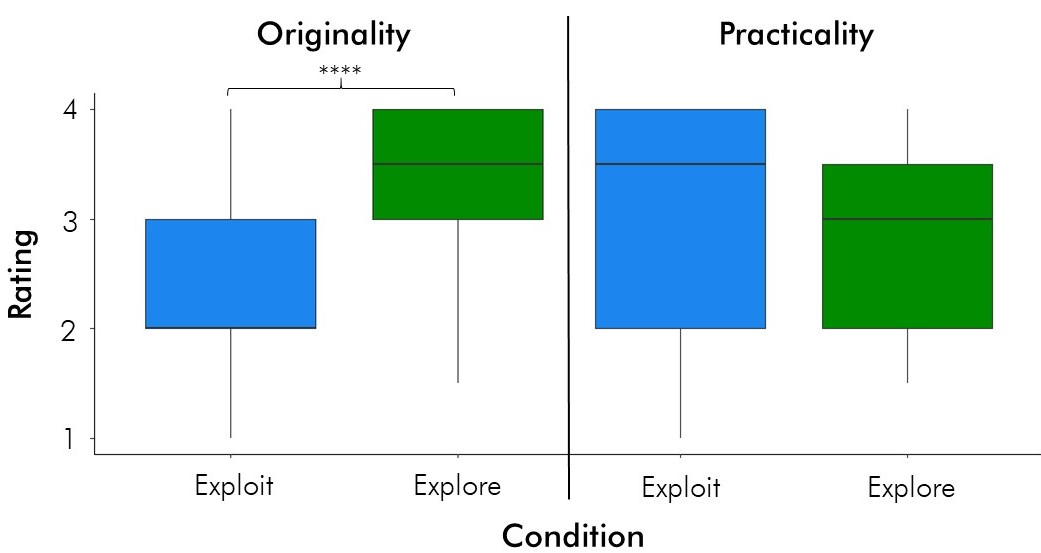
\includegraphics[width=\textwidth]{future/figures/baseline.jpg}
  \caption{Participants with the \textit{Explore} framing ($n=17$) received significantly higher originality ratings for their designs than the \textit{Exploit} framing ($n=17$). There were no significant differences between practicality ratings. ****$F(1,48)=15.2, R^2=0.22, p<.001$
}
  \label{fig:baseline}
\end{figure}

\subsubsection{Exploratory Framing Leads to More Original Designs \& More Diverse Ideas}
Two expert raters blind to condition with knowledge of campus issues and dining spaces rated each design on a 4-point Likert Scale for \textit{originality, practicality}, and \textit{justification} (how well motivated the design is). The inter-rater reliability between raters was substantial (${\kappa}=0.61$) Ratings were averaged between both raters for originality and practicality. \textit{Explore} condition designs received significantly higher average ratings for originality ($m=3.3, SD=0.75$) than \textit{Exploit} condition designs ($m=2.4, SD=0.88$)($F(1,48)=15.2, R^2=0.22, p<.001$). Contrary to our hypothesis that the exploit scaffold would lead to higher practicality ratings, there were no significant differences between conditions for practicality ratings (\textit{Explore} $m=2.82, SD=0.86$; \textit{Exploit} $m=3.02, SD=0.93$)($F(1,48)=0.62, R^2=-0.01, p=.43$) between both conditions (Figure \ref{fig:baseline}). 

The expert raters also assessed the diversity of each participant's ideas on a 4-point Likert scale. Highly similar ideas (\textit{i.e.} ``make buffet-style payment system,'' ``give students a certain number of swipes on payment cards'') earned a 1 while highly diverse ideas (\textit{i.e.} ``chefs for students included in tuition,'' ``grocery buddies/cooking mentors'') earned a 4 on this scale. \textit{Explore} participants ($m=3.02, SD=1.05$) brainstormed significantly more diverse ideas than \textit{Exploit} participants ($m=2.04, SD=0.99$)($F(1,48)=11.6, R^2=0.18, p<.005$) (Figure \ref{fig:diversity}). 

\begin{figure}[b!]
\centering
  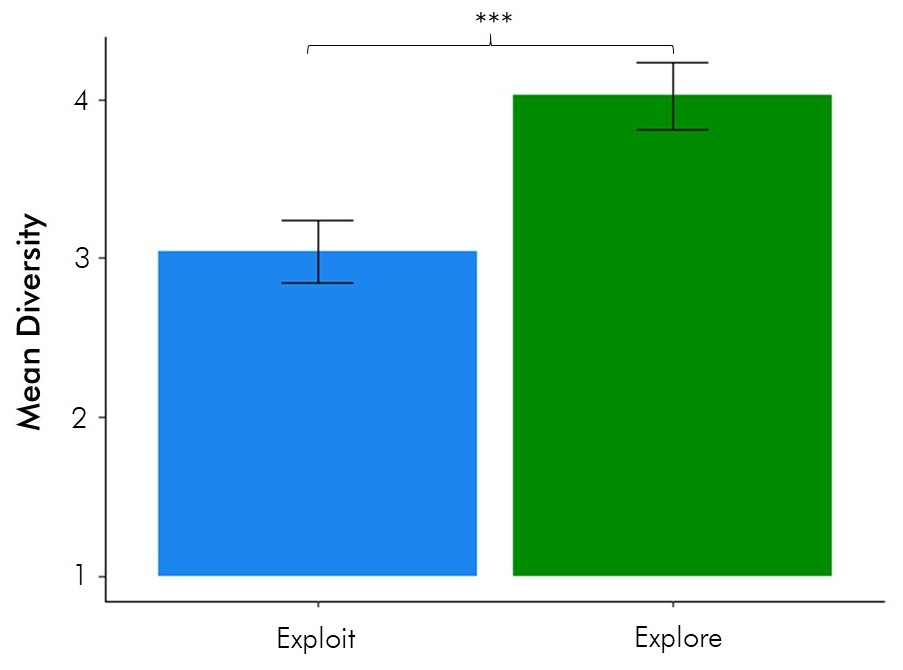
\includegraphics[width=.7\textwidth]{future/figures/diff.jpg}
  \caption{Participants with the \textit{Explore} ($n=17$) framing demonstrated greater diversity in their brainstormed ideas than those with the \textit{Exploit} ($n=17$) framing. ***$F(1,48)=11.6, R^2=0.18, p<.005$
}
  \label{fig:diversity}
\end{figure}

\subsubsection{Exploratory Framing Enhances Perceptions of Creativity}
The explore scaffold particularly helped participants push their boundaries of thought. One \textit{Explore} participant stated that the without the Thinking Hat, \textit{``I may have gotten to the same ideas..., but I probably would have refuted them on the spot with a reality check, or doubt.''} Another stated that the scaffold \textit{``made me question myself and think harder about the possibilities}.'' Two participants mentioned that the Thinking Hat as a metaphor was a particularly helpful metaphor. One participant said, \textit{``The green hat had a placebo effect on me..., which influenced me to think outside the box and use my creativity regardless of feasibility.''} Another stated that, \textit{``I could actually visualize wearing the hat [while] brainstorming new ideas.''} One participant even said the thinking hat itself served as inspiration for his design. 

\subsubsection{Exploit Framing Encourages Real-World Action}
Eight \textit{Exploit} participants mentioned that the problem frame scaffold helped with organizing and structuring their thoughts towards goal-oriented solutions. One \textit{Exploit} participant said the scaffold \textit{''made me think about how [my ideas] could be practically accomplished, since it seemed to emphasize real-world action.''} The exploit scaffold also seemed to be similar to participants' existing problem-solving strategies. Four participants believed their process of problem-solving without the thinking hat would have been the same. As one participant said, \textit{``I think the blue thinking hat already describes my thinking process..., so I didn't have to constantly remind myself to think a certain way or use different methods to think.''} None of the \textit{Exploit} participants mentioned that the scaffold was challenging; they all felt that it added or supplemented their ideation. However, one \textit{Exploit} participant felt the framing limited his thinking, stating that it ``\textit{restricted him to analytical thinking versus being creative.''}

\subsection{Experiment 2: Does the Order of Explore \& Exploit Affect Creative Outcomes?}
\subsubsection{Method}
A second experiment examined whether the order of the explore and exploit problem framing would impact creative outcomes. In this between-subjects study, 48 participants (30 female) from a California research university were recruited from an undergraduate design course. Similar to the first experiment, participants redesigned an aspect of the student eating experience. The task consisted of two initial brainstorming phases where participants used either explore or exploit scaffolds, the order of which was randomly counter-balanced between participants (23 participants in the \textit{Explore-Exploit} condition, 25 participants in the \textit{Exploit-Explore} condition). After each brainstorming phase, participants wrote a design idea, with the second design idea being the final design. Participants answered general questions about their experience in a post-survey after the experiment. 

%Don't center
% Participants in the Explore-Exploit condition (n=xx) were given the Explore prompt during brainstorming first while participants in the Exploit-Explore condition (n=xx) were given the Exploit prompt during brainstorming first. 

\subsubsection{Explore Framing Improved Originality of First Design}
Two experts in the food service industry blind to condition rated the final designs on two dimensions of \textit{Originality} and \textit{Practicality}, each on a 4-point Likert scale. Scores for each time point were averaged between both raters. The inter-rater reliability for raters was substantial (${\kappa}=0.69$). \textit{Explore-Exploit} participants received higher average originality ratings for their first design than \textit{Exploit-Explore} participants ($F(1,46)=8.1, R^2=0.13, p<.01$). There were no significant differences in originality ratings between conditions for the second design ($F(1,46)=1.08, R^2=.002, p=.30$). There were also no significant differences in practicality ratings between conditions for both the first ($F(1,46)=0.32, R^2=-0.01, p=.58$) and second designs ($F(1,46)=0.15, R^2=0.02, p=.70$)(Figure \ref{fig:order}). As this work is preliminary, our results suggest a trend for further investigation.

\subsubsection{Exploratory Scaffold Encouraged Wild Ideas}
Despite our observed null quantitative results for most measures, the explore scaffold seemed successful in challenging participants to think more creatively based on qualitative reports. One participant in the \textit{Explore-Exploit} condition noted, \textit{``it pushed me to think of designs from different perspectives and points of view.''} Similarly, one participant in the \textit{Exploit-Explore} condition thought the explore scaffold \textit{``opened the gates to better, more refined ideas.''} 

\begin{figure}
\centering
  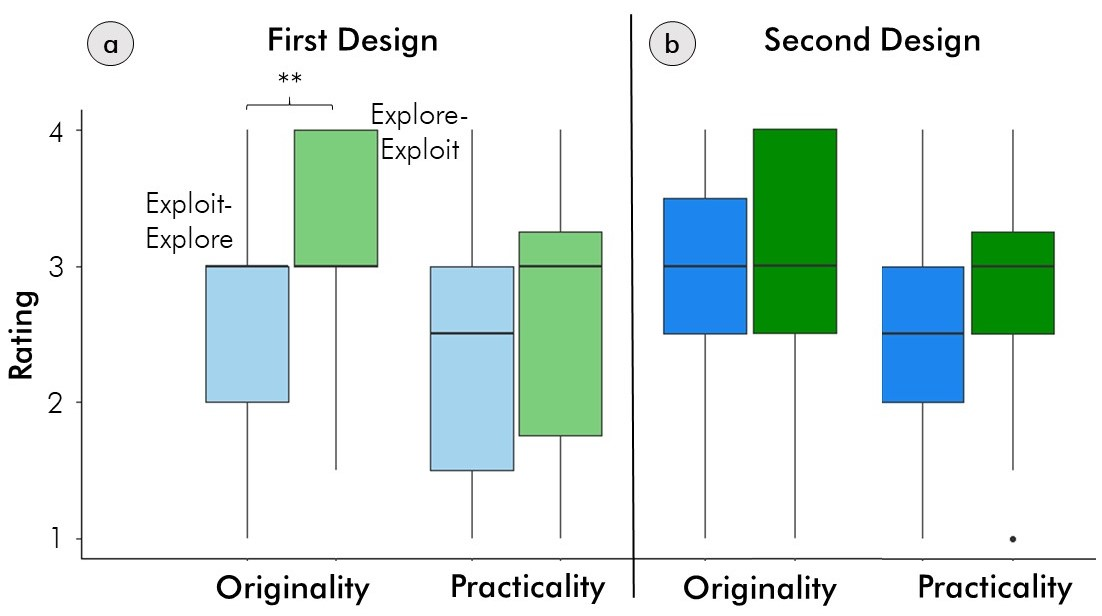
\includegraphics[width=.9\textwidth]{future/figures/order.jpg}
  \caption[a) Participants with the \textit{Explore-Exploit} order ($n=23$) received higher originality ratings for their first designs than \textit{Exploit-Explore} ($n=25$) participants, but not differences in practicality ratings.]{a) Participants with the \textit{Explore-Exploit} order ($n=23$) received higher originality ratings for their first designs than \textit{Exploit-Explore} ($n=25$) participants, but not differences in practicality ratings. b) We observed no significant differences in design outcomes for either measure in the second designs. A larger sample size or a change to the scaffolds themselves might result in more pronounced effects. **$F(1,46)=8.1, R^2=0.13, p<.01$
}
  \label{fig:order}
\end{figure}

Some participants in both conditions thought the explore scaffold was challenging, but ultimately useful for creativity. For example, one \textit{Explore-Exploit} participant said, \textit{``it was shocking, but after the initial shock it helped spur a lot more creative ideas.''} A participant in the \textit{Exploit-Explore} condition added, \textit{``it forced me to step outside of my comfort zone and see things from a different perspective even if I didn't think that was possible.''} This notion of feeling challenged may enhance creative thought regardless of order. 
\subsection{General Discussion \& Next Steps}
We provide preliminary empirical evidence of how problem framing can nudge people towards different cognitive processes and creative outcomes. This section addresses the implications and ongoing challenges of using this strategy.

\subsubsection{Exploring Broadly is Difficult Without Prerequisite Domain Knowledge}

The inclination to satisfice and find the ``good enough'' solution is particularly strong because of the time saved and effort required \cite{simon1972theories}. In both our experiments, the metaphor of an exploratory Thinking Hat seemed to enhance people's perceptions of their own creativity, which is a promising direction towards increasing productive exploration. Still, many final designs in Experiment 1 were similar to each other across conditions (for example, six designs mentioned sending out surveys for greater variety in dining halls on campus. Unfamiliarity with the domain space and the potential possibilities may have limited novices' ability to come up with fully original ideas. 

Importantly, the explore scaffolds led to increased intra-exploration, where people's ideas during brainstorming were more diverse even if their final design outcome was similar to others. In Experiment 1, \textit{Exploit} participants often came up with highly similar ideas or multiple examples of a single idea. In both experiments, participants frequently reported that the exploit scaffold was useful in structuring their thoughts, but it did not particularly challenge them to think differently. In contrast, many participants found the exploratory framing either challenging or effective in spurring new ideas. It may be that the perception or safety of feeling challenged enhances originality. Additionally, wearing even a metaphorical hat may enable people to play out a ``role'' of exploration or exploitation, similar to prior work on human-centered mindsets \cite{chou2017finding,teevan2017}. Our findings demonstrate that drawing attention to phase (explore or exploit) can influence creative mindset and potentially help in overcoming this tendency to satisfice and exploit early. An interesting area of future study might be examining how to further leverage this intra-exploration, perhaps by explicitly prompting for different perspectives or adding additional problem constraints.

\subsubsection{Early Exploration Can Lead to Better Exploitation}
Despite our hypothesis that a goal-oriented framing would lead to more practical ideas than the exploratory framing, we found no significant differences between the two conditions in both experiments. One potential concern of over-exploration is that wild ideas are produced without any being of practical use. Instead, broad exploration may help people realize the boundaries of a solution space without sacrificing practicality. We found this in Experiment 2 as well. Regardless of order, attending to exploration as a phase seemed fruitful in spurring more creative thought and ideas. 

Exploration may also lead to more concrete and specific ideas. Four designs in the \textit{Exploit} condition of Experiment 1 were overly broad. For example, one design suggested lowering the cost of food as a way to improve the student eating experience. While the design was well justified, it lacked specific details of how it could be put in place. An early exploration phase may indeed be necessary to refine concrete ideas later. This phase might attune people towards originality while maintaining their ability to later further develop and evaluate ideas. Future work should examine how to better scaffold the evaluation process to harness both unique and actionable ideas.

In Experiment 2, we observed that the \textit{Explore-Exploit} condition produced more original first designs with \textit{Exploit-Explore} participants improving slightly in Originality ratings for their second design. This may suggest that prompting for exploration is beneficial regardless of where the person is in their creative process. Just as semantically diverse examples provide the most creative inspiration when a person reaches an impasse \cite{chan2017semantically}, prompts for exploration might be most useful when a person feels stuck or ``out of ideas.'' Interestingly, a simple nudge, while not significant on its own, can at least catalyze getting unstuck.

\subsubsection{What Scaffolds Improve Exploration?}
Creative thinking combines domain knowledge with procedural strategies for greater exploration. Our experiments examine the latter, and our results suggest that how problems are framed affect people's thinking in different ways. Even simple metaphorical scaffolds like the Thinking Hats may be useful strategies in preparing novices to be creative by assigning a ``role'' to be creative. However, novices lack domain knowledge about a problem space and may need further help in understanding what creative means in a particular domain. To supplement this lack of knowledge, examples can provide anchors that usefully constrain a problem space \cite{Dow2009, kulkarni2012early}. Pairing problem framing as an exploratory strategy with the use of examples may aid in eliciting more creative design outcomes. In addition, combining problem framing with more structured exploratory strategies, such as those provided at the Stanford dschool (www.dschool.stanford.edu), can be an effective pedagogical approach for creative learning. 

\subsubsection{Summary}
%summarize experiments and what to do next
We present empirical results of how the framing of problems can ``set the temperature'' of creative thinking. We found that an exploratory framing leads to more diverse ideas and more original design outcomes. The explore scaffold challenged participants to think more freely about a problem; the exploit scaffold helped participants structure and organize their thoughts. Future work should examine how such problem framing can be used with other strategies and scaffolds to catalyze creative learning.

\subsubsection{Acknowledgements}
We thank research assistants Michelle Lee and Nicolas La Polla, study participants, and expert raters. This work was funded in part by NSF award \#1735234.

This chapter, in part, is currently being prepared for submission for publication of the material by Tricia J. Ngoon, Vivian Leung, and Caren M. Walker. The dissertation author was the primary investigator and author of this material.

This chapter, in part, includes portions of material as it appears in \textit{The Dark Side of Satisficing: Setting the Temperature of Creative Thinking} by Tricia J. Ngoon, Caren M. Walker, and Scott Klemmer in the Proceedings of the 2019 ACM Conference on Creativity and Cognition (C\&C '19). The dissertation author was the primary investigator and author of this material.